
% Preamble
\documentclass[12pt, letterpaper]{article}
\title{Chapter 2 - A Mathematical Representation of Waves - Notes}
\author{Jordan Tucker}
\date{April 4, 2026}
% Packages
\usepackage{amsmath}
\usepackage{parskip}
\usepackage{tabularx}
\usepackage{graphicx}
\usepackage{hyperref} %LaTeX package to import graphics
\graphicspath{{images/}} %configuring the graphicx package

% Document
\begin{document}
    \maketitle

    \section{A Mathematical Representation of Waves}
    The purpose of this chapter is to illustrate the use of functions of two variables as a way of
    representing and visualizing waves moving in a one-dimensional medium.
    We will only be looking at waves of one dimension.
    That is, the waves we are looking at might distort the medium along several dimensions, but they
    will always propagate and travel along a single dimension.

    \subsection{Representation of one-dimensional waves}
    A wave can be represented by a function $u(x,t)$ where \textit{x} is position and \textit{t} is
    time.
    If we fix $t_0$, we can look at $u$ as just a function of $x$.
    This allows us to easily identify any disturbances is our system (ex we might see a bump,
    extreme points, or abrupt changes).
    We can then fix different values of ${t_1, t_2, t_3, \dots, t_n}$ to see how that disturbance
    moves with time.

    \begin{figure}[h]
        \centering
        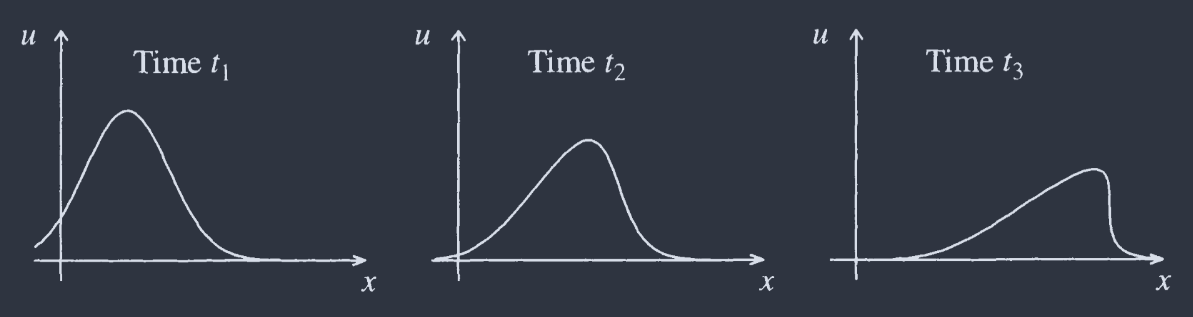
\includegraphics[width=0.75\textwidth]{disturbance}
        \caption{A graphical representation of a disturbance moving through a medium.}
    \end{figure}

    \textbf{Exercise 2.1.} Suppose that at time $t$, the value of $u$ at position $x$ in a
    one-dimensional medium is given by $u(x,t) = e^{-(x-t)^2}$.
    Snapshots of the wave represented by this function at times $t = 0, 1, 2, 3$ are

    \begin{center}
        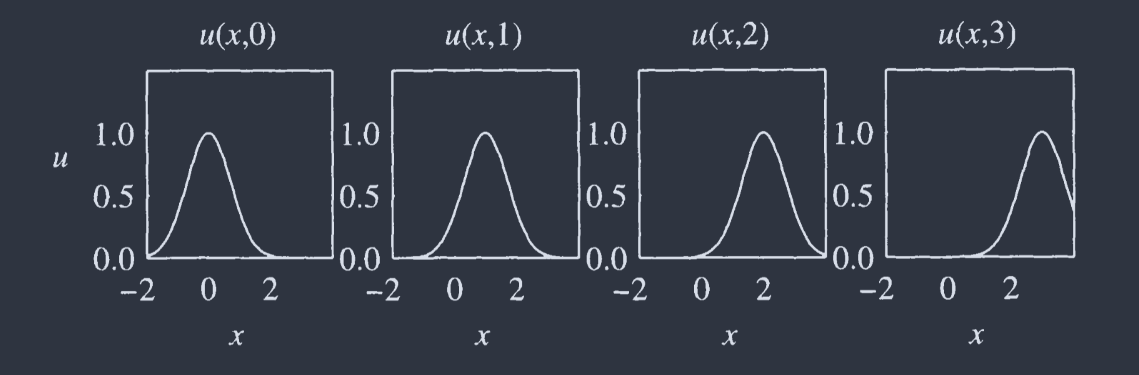
\includegraphics[width=0.8\textwidth]{exercise2-1}
    \end{center}

    and illustrate a wave moving right with constant speed.
    Modify the function $u(x,t)$ so that
    \begin{enumerate}
        \item[(a)] The wave moves to the left.
        \item[(b)] The wave moves to the right with increasing speed.
        \item[(c)] The amplitude (height) of the wave decreases as the wave moves to the right.
    \end{enumerate}
    Solution: \url{http://desmos.com/calculator/b07fhkpydc}

\end{document}